\documentclass[11pt,a4paper]{scrartcl}


\usepackage[utf8]{inputenc}
\usepackage[ngerman]{babel}
\usepackage{amsmath}
\usepackage{amssymb}
\usepackage{graphicx}
\usepackage{hyperref}
\usepackage{gauss}
\usepackage{stmaryrd}

\renewcommand{\thesubsection}{Exercise \arabic{section}.\arabic{subsection}}
\renewcommand{\thesubsubsection}{(\alph{subsubsection})}
\begin{document}
\author{Pavankumar Deshpande, Dmitrii Panichev, Paul Kröpke, Daniel Biskup}
\title{Foundations of Audio Signal Processing:}
\subtitle{Exercise sheet 2}
\maketitle

\setcounter{section}{3} %sheet 3
\subsection{} %3.1
Use:
\begin{align}
a+bi\\
r=\sqrt{a^2+b^2}\\
\cos(\varphi)=\frac{a}{r}\\
\sin(\varphi)=\frac{b}{r}
\end{align}
\subsubsection{} %a
\begin{align}
r=\sqrt{4^2+(4\sqrt{3})^2}=\sqrt{16+16*3}=\sqrt{64}=8\\
\cos(\varphi)=\frac{4}{8}=\frac{1}{2}\\
\sin(\varphi)=\frac{4\sqrt{3}}{8}=\frac{\sqrt{3}}{2}
\end{align}
Fulfilled by $\varphi = \frac{\pi}{3}$. Concluding: 
\begin{align}
4+i4\sqrt{3} = 8e^{i\pi/3}
\end{align}

\subsubsection{} %b
\begin{align}
r=\sqrt{(-1)^2+\sqrt{3}^2}=\sqrt{1+3}=\sqrt{4}=2\\
\cos(\varphi)=\frac{-1}{2}\\
\sin(\varphi)=\frac{\sqrt{3}}{2}\\
\end{align}
Fulfilled by $\varphi = \frac{2\pi}{3}$. Concluding: 
\begin{align}
(-1+i\sqrt{3})^4= (2e^{i2\pi/3})^4=16e^{i8\pi/3}\quad\overset{\text{periodicity}}{=}16e^{i2\pi/3}
\end{align}

\subsubsection{} %c
\begin{align}
\frac{(-1+i\sqrt{3})^4}{4++4\sqrt{3}}=\frac{8e^{i\pi/3}}{16e^{i2\pi/3}}=\frac{1}{2}e^{-i\pi/3}\quad\overset{\text{periodicity}}{=}\frac{1}{2}e^{i5\pi/3}
\end{align}

\subsubsection{} %d
Compute (1+i) first:
\begin{align}
r=\sqrt{2}\\
\cos(\varphi)=\frac{1}{\sqrt{2}}\\
\sin(\varphi)=\frac{1}{\sqrt{2}}
\end{align}
Fulfilled by $\varphi = \frac{\pi}{4}$. So $(1+i)=\sqrt{2}e^{i\pi/4}$. Computing the original exercise:
\begin{align}
2e^{i\pi/2}\cdot\sqrt{2}e^{i\pi/4}=2\sqrt{2}e^{i3\pi/4}
\end{align}
\newpage
\subsection{}
\subsubsection{}
The following figures show the requested functions.
\begin{figure}[h]
\centering
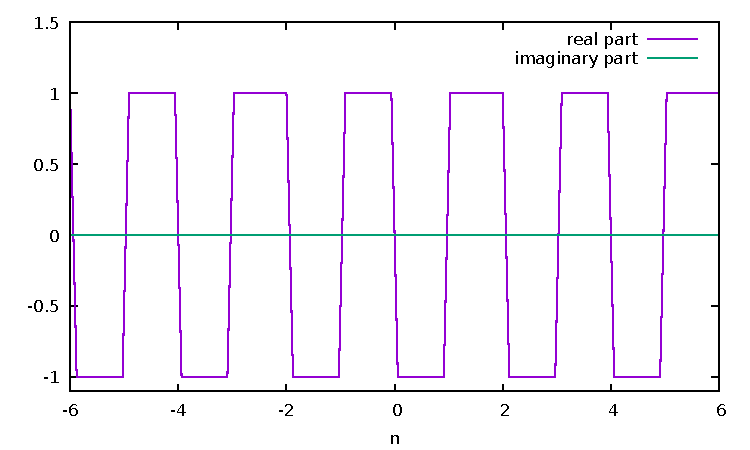
\includegraphics[width=10cm]{f2.pdf}
\label{f2}
\caption{$f_{1/2}(n)$}
\end{figure}

\begin{figure}[h]
\centering
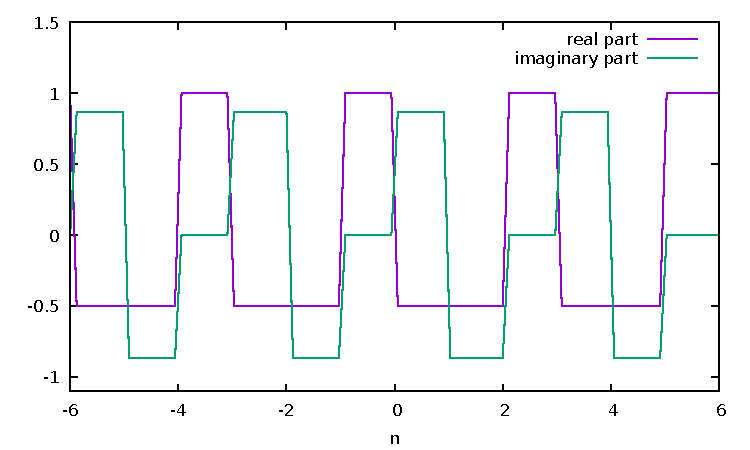
\includegraphics[width=10cm]{f3.pdf}
\label{f3}
\caption{$f_{1/3}(n)$}
\end{figure}

\newpage
\begin{figure}[h]
\centering
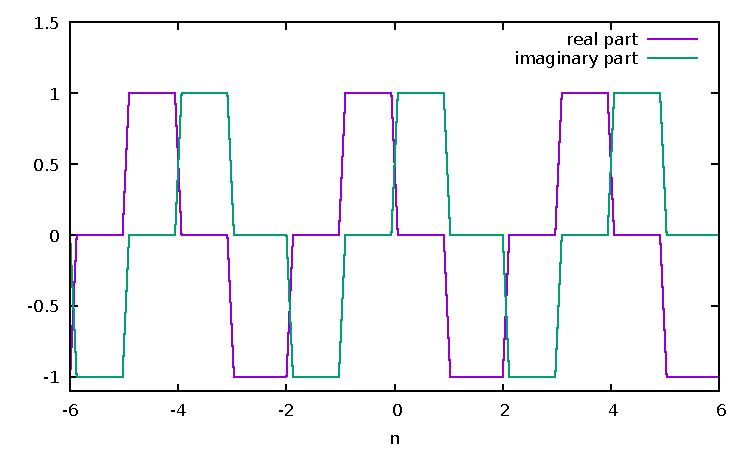
\includegraphics[width=10cm]{f4.pdf}
\label{f4}
\caption{$f_{1/4}(n)$}
\end{figure}

\begin{figure}[h]
\centering
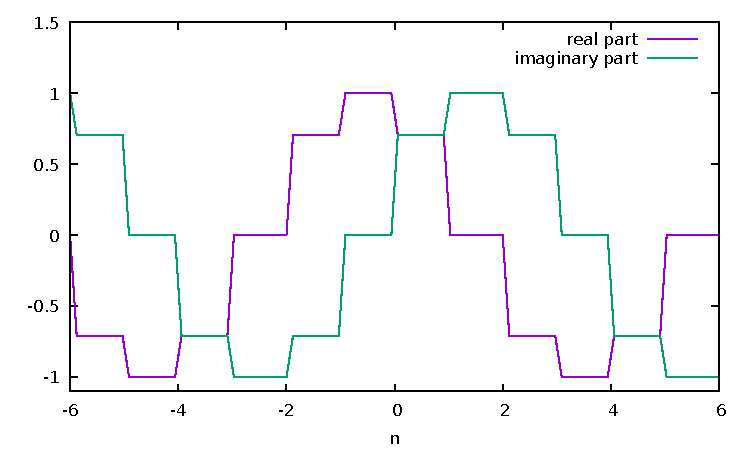
\includegraphics[width=10cm]{f8.pdf}
\label{f8}
\caption{$f_{1/8}(n)$}
\end{figure}

\subsubsection{}
\underline{"`$\Rightarrow$"':}
\begin{align}
f_\omega \text{ periodic}\quad\Rightarrow\quad \exists p\in\mathbb{N}: f_\omega(n+p)=f_\omega(n)\quad\forall n\in\mathbb{Z}\\
\Rightarrow \quad e^{2\pi i\omega (n+p)} = e^{2\pi i\omega (n+p)}\\
\Rightarrow \quad \cos(2\pi \omega (n+p)) + i\sin(2\pi \omega (n+p)) = \cos(2\pi \omega n) + i\sin(2\pi \omega n)\\
\overset{\text{cos and sin are periodic with period }2\pi}{\Rightarrow}\exists k\in\mathbb{Z}:\quad2\pi \omega (n+p) - 2\pi \omega n\overset{!}{=}k2\pi\\
\Rightarrow \quad \omega p = k \quad\Rightarrow\quad \omega = \dfrac{k}{p}\quad \Rightarrow \quad\omega\in\mathbb{Q}
\end{align}

\underline{"`$\Leftarrow$"':}
\begin{align}
\omega\in\mathbb{Q}\quad\Rightarrow\quad\exists q\in\mathbb{Z}, r\in\mathbb{N}: \omega = \dfrac{q}{r}\quad \Rightarrow\quad \omega r=q\\
\Rightarrow\quad 2\pi\omega(n+r)-2\pi\omega n = q2\pi\quad\forall n\in\mathbb{Z}\quad \overset{\text{cos and sin are periodic with period }2\pi}{\Rightarrow}\\ 
\cos(2\pi \omega (n+r)) + i\sin(2\pi \omega (n+r)) = \cos(2\pi \omega n) + i\sin(2\pi \omega n)\\
\Rightarrow \quad e^{2\pi i\omega (n+r)} = e^{2\pi i\omega (n+r)}\\
f_\omega(n+p)=f_\omega(n)\quad\Rightarrow\quad f_\omega \text{ periodic}
\end{align}

\subsection{}
\begin{align}
\cos^3(x)=&\dfrac{1}{8}(e^{ix}+e^{-ix})^3=\dfrac{1}{8}(e^{ix}+e^{-ix})(e^{2ix}+2+e^{-2ix})\\
=&\dfrac{1}{8}(e^{3ix}+e^{ix}+2e^{ix}+2e{-ix}+e^{-ix}+e^{-3ix})\\
=&\dfrac{1}{4}\left[\dfrac{1}{2}(e^{i(3x)}+e^{-i(3x)})\right]+\dfrac{3}{4}\left[\dfrac{1}{2}(e^{ix}+e^{-ix})\right]\\
=&\dfrac{1}{4}\cos(3x)+\dfrac{3}{4}\cos(x)
\end{align}

\end{document}